\subsubsection{Mittlerer Atomabstand}
Der mittlere Atomabstand wird aus den Messdaten mithilfe eines Bildbearbeitungsprogramms bestimmt. Die Abbildung ist durch die Messung verzerrt, da die Piezoelemente nicht in allen Richtungen die gleiche Kalibrierung haben. Insgesamt kann dadurch auch eine Abweichung vom wirklichen Atomabstand entstanden sein.
\begin{figure}[H]
\centering
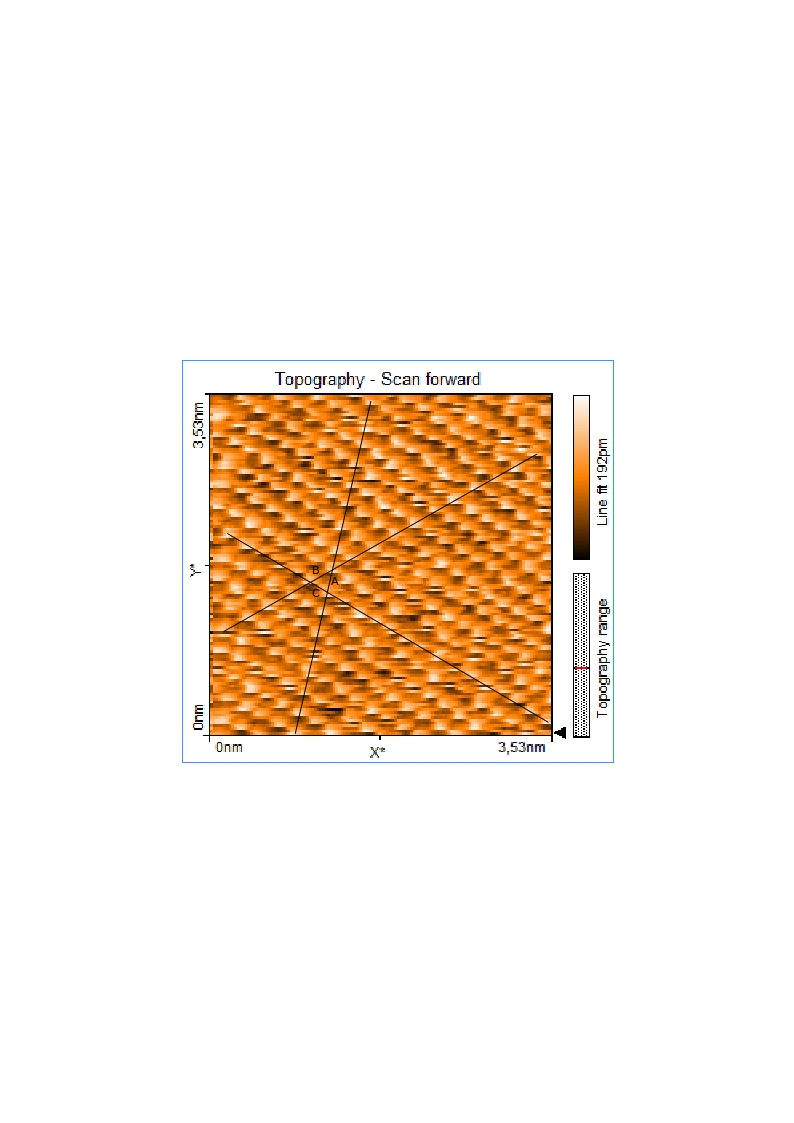
\includegraphics[trim = 10mm 120mm 10mm 125mm, clip=true, scale = 0.75]{ausschnitt_3_nanostruktur_2_bearbeitet.jpg}
\caption{ Bestimmung des mittleren Atomabstandes }
\label{fig:mittlerer_Atomabstand}
\end{figure}
Um den Atomabstand aus Abbildung \ref{fig:mittlerer_Atomabstand} zu bestimmen, werden die L�ngen von Linien parallel zu den eingezeichneten Linien gemessen und durch die Anzahl der Verbindungen von hellen Stellen geteilt.